\section{Saityno peržiūros roboto sistemos apžvalga}

Šiame skyriuje analizuojama teorinė saityno peržiūros roboto sistemų medžiaga, esminės funkcinės charakteristikos, nagrinėjamos skirtingos tokių sistemų kategorijos. Skyriaus medžiagos siekis -- sudaryti skaitytojui aiškesnį probleminės srities suvokimo kontekstą.

\subsection{Bazinis veikimo algoritmas}

Saityno peržiūros robotų sistemų funkcinis algoritmas nėra sudėtingas -- esminė tokių sistemų užduotis yra turint pradinį URL adresų sąrašą parsiųsti šių puslapių turinį naudojantis HTTP protokolu, iš parsiųstų HTML dokumentų išgauti hipernuorodas ir jas suabsoliutinus (nustačius ir resurso serverio vardą) pridėti į lankytinų nuorodų sąrašą tolesiam žvalgymui \cite{StanfWebCrawl}. Parsiųsti dokumentai saugomi didelėse saugyklose -- failinėse sistemose ar duomenų bazėse ir gali būti naudojami tolesniam papildomui aprodorimui (pvz.: svetainės indeksavimui ir semantiniam temos nustatymui, didžiųjų duomenų gavybai ir jų struktūrizavimui ar kt.)

\begin{figure}[ht]
\centering
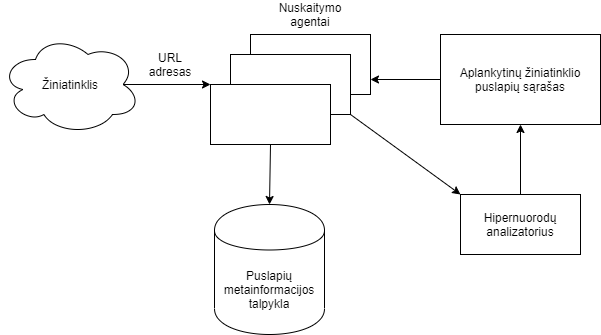
\includegraphics[scale=0.6]{img/Web_Crawler_Architecture.png}
\caption{Aukšto lygio saityno pežiūros roboto architektūra}
\label{fig:high_level_architecture}
\end{figure}
Supaprastinta abstrakti tokių sistemų veikimo schema pateikiama \ref{fig:high_level_architecture} paveikslėlyje. Taigi, iš schemos pastebimas ciklinis veikimo principas -- nuorodos analizuojamos nuolat iki kol ištuštėja lankytinų puslapių sąrašas arba inicijuojamas sistemos darbo nutraukimas iš vartotojo pusės. Tokios sistemos privalo pasižymėti aukštu lygegretaus agentų veikimo lygiu ir efektyviai išnaudoti sistemos tinklo, procesoriaus ir operatyviosios atminties resursus. Taip pat aktualus ir didelio kiekio duomenų talpinimo klausimas -- saugomi šimtai milijonų dokumentų ir nuorodų, o tai reikalauja didelių talpinimo resursų ir optimalios prieigos prie jų.

\pagebreak
\subsection{Palyginimas su saityno duomenų rinkimo sistemomis}
Terminai \textbf{saityno žvalgymas} (angl. \textit{Web Crawling}) ir \textbf{saityno duomenų rinkimas} (angl. \textit{Web Scraping}) dažnai vartojami kaip sinonimai nors jų reikšmės skiriasi. Siekiant įvesti aiškią skirtį ir apibrėžti darbe nagrinėjamo tipo sistemų funkcionalumo ribas, šiame skyriuje atliekamas terminų palyginimas. 

\subsubsection{Skirtumai}

Duomenų žvalgymas dažniausiai apima dideles saityno erdves -- vyksta tęstinis procesas, kurio metu siekiama identifikuoti puslapyje pasiekiamas hipernuorodas ir atlikti tų nuorodų tolimesnį žvalgymą. Tuo metu duomenų surinkimo sistema dažniausiai turi aiškų objektą ir jo struktūrą -- konkrečią svetainę ar duomenų bazę ir siekia išgauti tam tikrus dominančius duomenis. Galima teigti, jog saityno žvalgymo sistemos labiausiai suinteresuotos ryšių tarp puslapių nustatymui tam, kad būtų galima keliauti žiniatinkliu, o žiniatinklio duomenų surinkimo sistemų epicentre -- informacijos gavyba \cite{OxylabsScrapingVsCrawling}. \ref{tab:crawling_vs_scraping} lentelėje pateikta keletas esminių lyginamųjų charakteristikų tarp šių vartojamų terminų.
% Table generated by Excel2LaTeX from sheet 'crawling_vs_scraping'
\begin{table}[htbp]
  \centering
  \caption{Duomenų žvalgymo ir surinkimo sistemų palyginimas \cite{PromptCloudScrapingVsCrawling}}
    \begin{tabular}{|l|l|p{13.57em}|}
    \hline
    \textbf{Aspektas} & \textbf{Duomenų žvalgymas} & \textbf{Duomenų surinkimas} \bigstrut\\
    \hline
    Veikimo mastelis & Milžiniškas & Koncentruotas \bigstrut\\
    \hline
    Veikimo erdvė & Žiniatinklis & Žiniatinklis, duomenų bazė, serveris \bigstrut\\
    \hline
    Dublikatų aptikimas & Esminis veiksmas & Nebūtinas veiksmas \bigstrut\\
    \hline
    \multicolumn{1}{|p{12.285em}|}{Esminiai funkciniai komponentai} & Žvalgymo agentai & Žvalgymo agentai ir duomenų analizatoriai \bigstrut\\
    \hline
    Rankinio atlikimo galimybė & Negalima & Galima \bigstrut\\
    \hline
    Tikslas & Hipernuorodų aptikimas & Duomenų išgavimas \bigstrut\\
    \hline
    \end{tabular}%
  \label{tab:crawling_vs_scraping}%
\end{table}%

Nagrinėjami terminai skiriasi, tačiau yra itin susiję, nes saityno žvalgymas yra dažniausiai pirmasis informacijos gavybos etapas -- reikalingo turinio surinkimas. Žinoma, duomenų surinkimą galima atlikti be žvalgymo sistemų pagalbos, tačiau žvalgymo sistemos visada kartu naudoja duomenų surinkimo sistemas tam, kad atskirtų vertingą turinį nuo prastos reputacijos svetainės. \cite{OxylabsScrapingVsCrawling}

Taigi, šiame darbe nagrinėjamos duomenų žvalgymo robotų, dar vadinamų vorais (angl. \textit{Web Spider Bot}), sistemos, kurios keliauja saitynu naudojantis išgaunamomis hipernuorodomis. Rašto darbe nėra aptariamas svetainės turinio duomenų apdorojimas, struktūrizuotos informacijos gavyba, nes tai nėra šių sistemų atsakomybės sritys.

\subsection{Pagrindinės sistemos elgsenos strategijos}
\subsection{Kategorizacija}